% SPDX-License-Identifier: CC-BY-SA-4.0
%
% Copyright (c) 2020 Philipp Le
%
% Except where otherwise noted, this work is licensed under a
% Creative Commons Attribution-ShareAlike 4.0 License.
%
% Please find the full copy of the licence at:
% https://creativecommons.org/licenses/by-sa/4.0/legalcode

\phantomsection
\addcontentsline{toc}{section}{Exercise 6}
\section*{Exercise 6}


%%%%%%%%%%%%%%%%%%%%%%%%%%%%%%%%%%%%%%%%%%%%%%%%%%%%%%%%%%%%%%%%%%%%%%%%%%%%%%%
\begin{question}[subtitle={IIR Filter}]
	The following IIR filter is given.
	\begin{figure}[H]
		\centering
		\begin{circuitikz}
			\draw[o-] (-1,0) node[left, align=right]{$\underline{x}[n]$} -- (0,0);
			\draw (0,-3) node[adder](Add1){};
			\draw (2,-3) node[adder](Add2){};
			\draw (0,0) to[amp,l=$\underline{b}_0$,>,-] (Add1.north) node[inputarrow,rotate=-90]{};
			\draw (0,0) to[short,*-] (2,0) to[twoport,t=$z^{-1}$,>,-] (Add2.north) node[inputarrow,rotate=-90]{};
			\draw (Add1.east) to[short] (Add2.west) node[inputarrow,rotate=0]{};
			\draw[-latex] (Add2.east) to[short] (4,-3) node[right, align=left]{$\underline{y}[n]$};
			\draw (3,-3) to[short,*-] (3,-6) to[twoport,t=$z^{-1}$,>,-] (0,-6) to[amp,l=$\underline{a}_0$,>,-] (Add1.south) node[inputarrow,rotate=90]{};
		\end{circuitikz}
	\end{figure}
	with:
	\begin{itemize}
		\item $\underline{a}_0 = 0.5$
		\item $\underline{b}_0 = 2$
	\end{itemize}
	
	\begin{tasks}
		\task
		Give the differential equation of the filter!
		\task
		Give the transfer function of the filter!
		\task
		How much is the filter order?
		\task
		Is the filter stable?
		\task
		Plot the amplitude and phase response between $0$ and $\pi$.
	\end{tasks}
\end{question}

\begin{solution}
	\begin{tasks}
		\task
		See hand-written solution
		
		\task
		See hand-written solution
		
		\task
		See hand-written solution
		
		\task
		See hand-written solution
		
		\task
		\begin{table}[H]
			\centering
			\begin{tabular}{|r|r|r|}
				\hline
				$\phi$ in \si{rad} & $\left|\underline{H}\left(e^{j\phi}\right)\right|$ & $\arg\left(\underline{H}\left(e^{j\phi}\right)\right)$ in \si{rad} \\
				\hline
				\hline
				$0$ & $2$ & $0$ \\
				\hline
				$0.39$ & $2$ & $0$ \\
				\hline
				$0.79$ & $2$ & $0$ \\
				\hline
				$1.18$ & $2$ & $0$ \\
				\hline
				$1.57$ & $2$ & $0$ \\
				\hline
				$1.96$ & $2$ & $0$ \\
				\hline
				$2.36$ & $2$ & $0$ \\
				\hline
				$2.75$ & $2$ & $0$ \\
				\hline
			\end{tabular}
		\end{table}
	
		\begin{figure}[H]
			\centering
			\begin{tikzpicture}
				\begin{axis}[
					height={0.10\textheight},
					width=0.7\linewidth,
					scale only axis,
					xlabel={$\phi$ in \si{rad}},
					ylabel={$\left|\underline{H}\left(e^{j\phi}\right)\right|$},
					%grid style={line width=.6pt, color=lightgray},
					%grid=both,
					grid=none,
					legend pos=north east,
					axis y line=middle,
					axis x line=middle,
					every axis x label/.style={
						at={(ticklabel* cs:1.05)},
						anchor=north,
					},
					every axis y label/.style={
						at={(ticklabel* cs:1.05)},
						anchor=east,
					},
					xmin=0,
					xmax=3.5,
					ymin=0,
					ymax=2.2,
					xtick={0, 1.5708, 3.14159},
					xticklabels={0, $\frac{\pi}{2}$, $\pi\hspace{0.10cm}$},
%					ytick={0},
				]
					\addplot[red] coordinates {(0, 2) (0.39, 2) (0.79, 2) (1.18, 2) (1.57, 2) (1.96, 2) (2.36, 2) (2.75, 2)};
				\end{axis}
			\end{tikzpicture}
		\end{figure}
	
		\begin{figure}[H]
			\centering
			\begin{tikzpicture}
				\begin{axis}[
				height={0.10\textheight},
				width=0.7\linewidth,
				scale only axis,
				xlabel={$\phi$ in \si{rad}},
				ylabel={$\arg\left(\underline{H}\left(e^{j\phi}\right)\right)$ in \si{rad}},
				%grid style={line width=.6pt, color=lightgray},
				%grid=both,
				grid=none,
				legend pos=north east,
				axis y line=middle,
				axis x line=middle,
				every axis x label/.style={
					at={(ticklabel* cs:1.05)},
					anchor=north,
				},
				every axis y label/.style={
					at={(ticklabel* cs:1.05)},
					anchor=east,
				},
				xmin=0,
				xmax=3.5,
				ymin=-3.5,
				ymax=3.5,
				xtick={0, 1.5708, 3.14159},
				xticklabels={0, $\frac{\pi}{2}$, $\pi\hspace{0.10cm}$},
				ytick={-3.14159, -1.5708, 0, 1.5708, 3.14159},
				yticklabels={$\pi\hspace{0.30cm}-$, $-\frac{\pi}{2}$, 0, $\frac{\pi}{2}$, $\pi\hspace{0.10cm}$},
			]
				\addplot[blue] coordinates {(0, 0) (0.39, 0) (0.79, 0) (1.18, 0) (1.57, 0) (1.96, 0) (2.36, 0) (2.75, 0)};
			\end{axis}
		\end{tikzpicture}
		\end{figure}
	\end{tasks}
\end{solution}


%%%%%%%%%%%%%%%%%%%%%%%%%%%%%%%%%%%%%%%%%%%%%%%%%%%%%%%%%%%%%%%%%%%%%%%%%%%%%%%
\begin{question}[subtitle={FIR Filter}]
	An FIR filter with following coefficients is given.
	\begin{itemize}
		\item $b_0 = 1$.
		\item $b_1 = 0.5 + j \cdot 1$.
		\item $b_2 = 2$.
	\end{itemize}

	The sampling rate of the digital system is \SI{2}{MHz}.
	
	\begin{tasks}
		\task
		Give the block diagram of the filter!
		\task
		Give the transfer function of the filter!
		\task
		Give the differential equation of the filter!
		\task
		How much is the filter order?
		\task
		Plot the amplitude and phase response between \SI{-1}{MHz} and \SI{1}{MHz}.
		\task
		Proof mathematically that all poles of the FIR filter are $0$!
	\end{tasks}
\end{question}

\begin{solution}
	\begin{tasks}
		\task
		See hand-written solution
		
		\task
		See hand-written solution
		
		\task
		See hand-written solution
		
		\task
		See hand-written solution
		
		\task
		\begin{table}[H]
			\centering
			\begin{tabular}{|r|r|r|}
				\hline
				$f$ in \si{kHz} & $\left|\underline{H}\left(e^{j\phi}\right)\right|$ & $\arg\left(\underline{H}\left(e^{j\phi}\right)\right)$ in \si{rad} \\
				\hline
				\hline
				$-875$ & $2.66222$ & $-0.940067$ \\
				\hline
				$-750$ & $2.35077$ & $-1.59632$ \\
				\hline
				$-625$ & $2.02726$ & $-2.42601$ \\
				\hline
				$-500$ & $2.06155$ & $2.89661$ \\
				\hline
				$-375$ & $2.53576$ & $2.0415$ \\
				\hline
				$-250$ & $3.12827$ & $1.36149$ \\
				\hline
				$-125$ & $3.54979$ & $0.793366$ \\
				\hline
				$0$ & $3.64005$ & $0.2783$ \\
				\hline
				$125$ & $3.33017$ & $-0.20564$ \\
				\hline
				$250$ & $2.63934$ & $-0.675333$ \\
				\hline
				$375$ & $1.64624$ & $-1.1316$ \\
				\hline
				$500$ & $0.5$ & $-1.5708$ \\
				\hline
				$625$ & $0.653682$ & $1.05924$ \\
				\hline
				$750$ & $1.64502$ & $0.608236$ \\
				\hline
				$875$ & $2.34923$ & $0.128051$ \\
				\hline
				$1000$ & $2.69258$ & $-0.380506$ \\
				\hline
			\end{tabular}
		\end{table}
	
		Amplitude and phase plots will not be symmetric, because one filter coefficient is complex-valued.
	
		\begin{figure}[H]
			\centering
			\begin{tikzpicture}
				\begin{axis}[
					height={0.10\textheight},
					width=0.7\linewidth,
					scale only axis,
					xlabel={$f$ in \si{Hz}},
					ylabel={$\left|\underline{H}\left(e^{j\phi}\right)\right|$},
					%grid style={line width=.6pt, color=lightgray},
					%grid=both,
					grid=none,
					legend pos=north east,
					axis y line=middle,
					axis x line=middle,
					every axis x label/.style={
						at={(ticklabel* cs:1.05)},
						anchor=north,
					},
					every axis y label/.style={
						at={(ticklabel* cs:1.05)},
						anchor=east,
					},
%					xmin=-3.5,
%					xmax=3.5,
					ymin=0,
					ymax=3.7,
%					xtick={0, 1.5708, 3.14159},
%					xticklabels={0, $\frac{\pi}{2}$, $\pi\hspace{0.10cm}$},
%					ytick={0},
				]
					\addplot[red] coordinates {(-875000, 2.66222) (-750000, 2.35077) (-625000, 2.02726) (-500000, 2.06155) (-375000, 2.53576) (-250000, 3.12827) (-125000, 3.54979) (0, 3.64005) (125000, 3.33017) (250000, 2.63934) (375000, 1.64624) (500000, 0.5) (625000, 0.653682) (750000, 1.64502) (875000, 2.34923) (1e+06, 2.69258)};
				\end{axis}
			\end{tikzpicture}
		\end{figure}
	
		\begin{figure}[H]
			\centering
			\begin{tikzpicture}
				\begin{axis}[
				height={0.10\textheight},
				width=0.7\linewidth,
				scale only axis,
				xlabel={$f$ in \si{Hz}},
				ylabel={$\arg\left(\underline{H}\left(e^{j\phi}\right)\right)$ in \si{rad}},
				%grid style={line width=.6pt, color=lightgray},
				%grid=both,
				grid=none,
				legend pos=north east,
				axis y line=middle,
				axis x line=middle,
				every axis x label/.style={
					at={(ticklabel* cs:1.05)},
					anchor=north,
				},
				every axis y label/.style={
					at={(ticklabel* cs:1.05)},
					anchor=east,
				},
%				xmin=-3.5,
%				xmax=3.5,
				ymin=-3.5,
				ymax=3.5,
%				xtick={0, 1.5708, 3.14159},
%				xticklabels={0, $\frac{\pi}{2}$, $\pi\hspace{0.10cm}$},
				ytick={-3.14159, -1.5708, 0, 1.5708, 3.14159},
				yticklabels={$\pi\hspace{0.30cm}-$, $-\frac{\pi}{2}$, 0, $\frac{\pi}{2}$, $\pi\hspace{0.10cm}$},
			]
				\addplot[blue] coordinates {(-875000, -0.940067) (-750000, -1.59632) (-625000, -2.42601) (-500000, 2.89661) (-375000, 2.0415) (-250000, 1.36149) (-125000, 0.793366) (0, 0.2783) (125000, -0.20564) (250000, -0.675333) (375000, -1.1316) (500000, -1.5708) (625000, 1.05924) (750000, 0.608236) (875000, 0.128051) (1e+06, -0.380506)};
			\end{axis}
		\end{tikzpicture}
		\end{figure}
		
		\task
		See hand-written solution
	\end{tasks}
\end{solution}


%%%%%%%%%%%%%%%%%%%%%%%%%%%%%%%%%%%%%%%%%%%%%%%%%%%%%%%%%%%%%%%%%%%%%%%%%%%%%%%
\begin{question}[subtitle={Down-sampling}]
	An analogue signal $x(t)$ is digitized (sampled and quantized).
	\begin{equation*}
		x(t) = \sin\left(2 \pi \cdot \SI{96}{kHz} \cdot t\right)
	\end{equation*}
	The signal has been sampled by a \SI{8}{bit}-ADC at \SI{7.68}{MHz}.
	
	The signal $x[n]$ is decimated by $N = 40$.
	
	\begin{tasks}
		\task
		How much is the sampling rate of the decimated signal?
		\task
		Is the signal suitable to be decimated by $N = 40$? Explain why! What is the criterion?
		\task
		What is the optimal sampling phase?
		\task
		Explain the effect on the spectrum caused by down-sampling!
		\task
		How much is the processing gain? How much is the effective number of bits?
	\end{tasks}
\end{question}

\begin{solution}
	\begin{tasks}
	\end{tasks}
\end{solution}


%%%%%%%%%%%%%%%%%%%%%%%%%%%%%%%%%%%%%%%%%%%%%%%%%%%%%%%%%%%%%%%%%%%%%%%%%%%%%%%
\begin{question}[subtitle={FFT}]
	A series of the samples in the time-domain is given:
	\begin{equation*}
		x[n] = \left[2, \underline{-0.5}, 1, -2 \right]
	\end{equation*}
	
	\begin{remark}
		The underline marks the sample at $n = 0$.
	\end{remark}
	
	\begin{tasks}
		\task
		Calculate the DFT for $k = 0, \ldots, 3$!
		\task
		Draw the butterfly graph of the Cooley-Tuckey FFT algorithm!
		\task
		Give the primitive roots of unity for each sub-FFT in the butterfly graph!
		\task
		Calculate the FFT using the Cooley-Tuckey FFT algorithm!
		\task
		Compare the number of multiply-accumulate operations necessary for both methods in a) and d)!
		\task
		\textit{(optional programming task)} Implement the FFT algorithm in a programming language of your choice!
	\end{tasks}
\end{question}

\begin{solution}
	The signal is periodic with $N = 4$. So, it can be re-written as:
	\begin{equation*}
		x[n] = \left[\underline{-0.5}, 1, -2, 2\right]
	\end{equation*}
	
	\begin{tasks}
		\task
		The formula of the DFT is:
		\begin{equation}
			\underline{X}[k] = \sum\limits_{n = 0}^{N - 1} \underline{x}[n] \cdot e^{- j \frac{2 \pi}{N} k n}
		\end{equation}
		where:
		\begin{itemize}
			\item $N = 4$
			\item $\underline{x}[0] = -0.5$
			\item $\underline{x}[1] = 1$
			\item $\underline{x}[2] = -2$
			\item $\underline{x}[3] = \underline{x}[-1] = 2$
		\end{itemize}
		
		\begin{equation*}
			\begin{split}
				\underline{X}[0] &= \underline{x}[0] \cdot e^{-j \frac{\pi}{2} 0 \cdot 0} + \underline{x}[1] \cdot e^{-j \frac{\pi}{2} 0 \cdot 1} + \underline{x}[2] \cdot e^{-j \frac{\pi}{2} 0 \cdot 2} + \underline{x}[3] \cdot e^{-j \frac{\pi}{2} 0 \cdot 3} = 0.5 \\
				\underline{X}[1] &= \underline{x}[0] \cdot e^{-j \frac{\pi}{2} 1 \cdot 0} + \underline{x}[1] \cdot e^{-j \frac{\pi}{2} 1 \cdot 1} + \underline{x}[2] \cdot e^{-j \frac{\pi}{2} 1 \cdot 2} + \underline{x}[3] \cdot e^{-j \frac{\pi}{2} 1 \cdot 3} = 1.5+1j \\
				\underline{X}[2] &= \underline{x}[0] \cdot e^{-j \frac{\pi}{2} 2 \cdot 0} + \underline{x}[1] \cdot e^{-j \frac{\pi}{2} 2 \cdot 1} + \underline{x}[2] \cdot e^{-j \frac{\pi}{2} 2 \cdot 2} + \underline{x}[3] \cdot e^{-j \frac{\pi}{2} 2 \cdot 3} = -5.5 \\
				\underline{X}[3] &= \underline{x}[0] \cdot e^{-j \frac{\pi}{2} 3 \cdot 0} + \underline{x}[1] \cdot e^{-j \frac{\pi}{2} 3 \cdot 1} + \underline{x}[2] \cdot e^{-j \frac{\pi}{2} 3 \cdot 2} + \underline{x}[3] \cdot e^{-j \frac{\pi}{2} 3 \cdot 3} = 1.5-1j
			\end{split}
		\end{equation*}
		
		\task
		\begin{figure}[H]
			\centering
			\begin{circuitikz}[
				x=0.4cm,
				y=0.4cm,
				littleamp/.style={amp, blocks/scale=0.2}
			]
				\pgfmathsetmacro{\Xscale}{5}
				\pgfmathsetmacro{\Cmargin}{0.15}
				
				\foreach \n/\f/\g in {0/1/3,1/0/2}{
					\draw (0,{((2*\n+1)*\Xscale)}) node[left,align=right]{$\underline{x}[\f]$} -- ({10-\Cmargin},{((2*\n+1)*\Xscale)}) node[inputarrow,rotate=0]{};
					\node[adder,scale=0.2] at(10,{(\n*2*\Xscale)+(\Xscale)}) {};
					\draw (0,{(\n*2*\Xscale)}) node[left,align=right]{$\underline{x}[\g]$}  -- (7.5,{(\n*2*\Xscale)}) to[littleamp,l=$\underline{w}_2^{1}$] ({10-\Cmargin},{(\n*2*\Xscale)}) node[inputarrow,rotate=0]{};
					\node[adder,scale=0.2] at(10,{(\n*2*\Xscale)}) {};
					\draw (5,{(\n*2*\Xscale)+\Xscale}) to[short,*-] ({10-\Cmargin},{(\n*2*\Xscale)+\Cmargin}) node[inputarrow,rotate=-45]{};
					\draw (5,{(\n*2*\Xscale)}) to[short,*-] (7.5,{(\n*2*\Xscale)+(\Xscale/2)}) to[littleamp,l=$\underline{w}_2^{0}$] ({10-\Cmargin},{(\n*2*\Xscale)+\Xscale-\Cmargin}) node[inputarrow,rotate=45]{};
				}
				\foreach \n/\g in {0/3,1/2}{
					\draw ({10+\Cmargin},{(\n*\Xscale)+(2*\Xscale)}) -- ({20-\Cmargin},{(\n*\Xscale)+(2*\Xscale)}) node[inputarrow,rotate=0]{};
					\node[adder,scale=0.2] at(20,{(\n*\Xscale)+(2*\Xscale)}) {};
					\draw ({10+\Cmargin},{(\n*\Xscale)}) -- (17.5,{(\n*\Xscale)}) to[littleamp,l=$\underline{w}_4^{\g}$] ({20-\Cmargin},{(\n*\Xscale)}) node[inputarrow,rotate=0]{};
					\node[adder,scale=0.2] at(20,{(\n*\Xscale)}) {};
				}
				\foreach \n/\g in {0/1,1/0}{
					\draw (15,{(2*\Xscale)+(\n*\Xscale)}) node[above,align=center,red]{$\underline{E}[\g]$} to[short,*-] ({20-\Cmargin},{(\n*\Xscale)+\Cmargin}) node[inputarrow,rotate=-60]{};
					\draw (15,{(\n*\Xscale)}) node[below,align=center,red]{$\underline{O}[\g]$} to[short,*-] (17.5,{(\Xscale)+(\n*\Xscale)}) to[littleamp,l=$\underline{w}_4^{\g}$] ({20-\Cmargin},{(2*\Xscale)+(\n*\Xscale)-\Cmargin}) node[inputarrow,rotate=60]{};
				}
				\foreach \f in {0,1,2,3}{
					\draw ({20+\Cmargin},{(3-\f)*\Xscale}) -- (25,{(3-\f)*\Xscale}) node[inputarrow,rotate=0]{} node[right,align=left]{$\underline{X}[\f]$};
				}
				\foreach \n in {1,5}{
					\draw[dashed] (3.5,{(\Xscale*\n/2)+3.5}) -- (3.5,{(\Xscale*\n/2)-3.5}) -- (11.5,{(\Xscale*\n/2)-3.5}) -- (11.5,{(\Xscale*\n/2)+3.5}) node[above left,align=right]{2-point FFT} -- cycle;
				}
			\end{circuitikz}
		\end{figure}
	
		The 4-point DFT can divided into two 2-point DFTs and a 4-point combination network (butterfly graph). The 2-point sub-DFTs are itself two 1-point DFTs and a 2-point combination network (butterfly graph). Ordering by even and odd indices must be considered.
		
		\task
		The unit circle is equally divided by the primitive roots of unity.
		\begin{equation}
			\underline{w}_N = e^{- j \frac{2 \pi}{N}}
		\end{equation}
		
		$N$ is the number of points of the FFT. $N$ must be a power of $2$, i.e., $1$, $2$, $4$, $8$, $16$, $32$, ..., $512$, $1024$, ...
		
		\begin{itemize}
			\item The primitive root of unity of the 2-point DFT ($N = 2$)
			\begin{equation*}
				\underline{w}_2 = e^{- j \pi}
			\end{equation*}
			\item The primitive root of unity of the 4-point DFT ($N = 4$)
			\begin{equation*}
				\underline{w}_4 = e^{- j \frac{\pi}{2}}
			\end{equation*}
		\end{itemize}
	
		\task
		At first, calculate the two 2-point sub-FFTs, called \emph{even} part ($\underline{E}[k]$) and \emph{odd} part ($\underline{O}[k]$).
		\begin{equation*}
			\begin{split}
				\underline{E}[0] &= \underline{x}[0] + \underline{w}_2^{0} \cdot \underline{x}[2] = -2.5 \\
				\underline{E}[1] &= \underline{x}[0] + \underline{w}_2^{1} \cdot \underline{x}[2] = 1.5 \\
				\underline{O}[0] &= \underline{x}[1] + \underline{w}_2^{0} \cdot \underline{x}[3] = 3.0 \\
				\underline{O}[1] &= \underline{x}[1] + \underline{w}_2^{1} \cdot \underline{x}[3] = -1.0
			\end{split}
		\end{equation*}
		Note that both $\underline{E}[k]$ and $\underline{O}[k]$ are 2-periodic, i.e., $\underline{E}[2] = \underline{E}[0]$, ...
		
		Now combine the two parts, to the 4-point FFT.
		\begin{equation*}
			\begin{split}
				\underline{X}[0] &= \underline{E}[0] + \underline{w}_4^{0} \cdot \underline{O}[0] = 0.5 \\
				\underline{X}[1] &= \underline{E}[1] + \underline{w}_4^{1} \cdot \underline{O}[1] = 1.5+1j \\
				\underline{X}[2] &= \underline{E}[0] + \underline{w}_4^{2} \cdot \underline{O}[0] = -5.5 \\
				\underline{X}[3] &= \underline{E}[1] + \underline{w}_4^{3} \cdot \underline{O}[1] = (1.5-1j)
			\end{split}
		\end{equation*}
		
		The result is the same like in a).
		
		\task
		\begin{itemize}
			\item a) and d) gave the same results. They both calculate the DFT.
			\item a) required 16 multiplications.
			\item d) required only 8 multiplications.
			\item Multiplications require many computational resources. d) will perform better, because it requires fewer multiplications.
		\end{itemize}
		
	\end{tasks}
\end{solution}

%%%%%%%%%%%%%%%%%%%%%%%%%%%%%%%%%%%%%%%%%%%%%%%%%%%%%%%%%%%%%%%%%%%%%%%%%%%%%%%
%\begin{question}[subtitle={Decibel}]
%	\begin{tasks}
%	\end{tasks}
%\end{question}
%
%\begin{solution}
%	\begin{tasks}
%	\end{tasks}
%\end{solution}
